%==============================================================================
%  Hardware-Aware Quantum Bayesian Learner Compression  —  QCE26 Poster
%  36 in (W) x 48 in (H) portrait, 3 columns, Duke-branded, beamerposter
%==============================================================================
\documentclass[final]{beamer}
\usepackage[orientation=portrait,size=custom,width=91.44,height=121.92,scale=1.25]{beamerposter}

\usepackage[T1]{fontenc}
\usepackage[utf8]{inputenc}
\usepackage{helvet}
\renewcommand{\familydefault}{\sfdefault}
\usepackage{microtype}
\usepackage{graphicx}
\usepackage{amsmath,amssymb}
\usepackage{booktabs}
\usepackage{colortbl}
\usepackage{array}
\usepackage{tcolorbox}
\tcbuselibrary{skins}
\usepackage{tikz}
\usetikzlibrary{calc}
\usepackage[absolute,overlay]{textpos}

%------------------------------------------------------------------ colors
\definecolor{dukenavy}{HTML}{012169}
\definecolor{dukeroyal}{HTML}{00539B}
\definecolor{dukeamber}{HTML}{E89923}
\definecolor{boxtint}{HTML}{EEF2F8}
\definecolor{inkblack}{HTML}{1A1A1A}
\definecolor{rulegray}{HTML}{C7D2E0}

%------------------------------------------------------------------ beamer theme stripping
\setbeamertemplate{navigation symbols}{}
\setbeamercolor{background canvas}{bg=white}
\setbeamercolor{normal text}{fg=inkblack}
\usebeamercolor[fg]{normal text}

% kill default block styling (we use tcolorbox)
\setbeamertemplate{itemize items}[triangle]
\setbeamercolor{itemize item}{fg=dukeroyal}
\setbeamercolor{itemize subitem}{fg=dukeroyal}

%------------------------------------------------------------------ geometry helpers
\newlength{\colw}
\setlength{\colw}{27.6cm}      % column width (~10.9 in)
\newlength{\sepw}
\setlength{\sepw}{3.0cm}       % gutter

%------------------------------------------------------------------ section header bar
% \secbar{number}{Title}
\newcommand{\secbar}[2]{%
  \vspace{0.15ex}%
  \begin{tcolorbox}[
      enhanced, sharp corners, boxrule=0pt, frame hidden,
      colback=dukenavy, left=10pt, right=10pt, top=7pt, bottom=7pt,
      width=\linewidth, before skip=4pt, after skip=8pt]
    \color{white}\bfseries\large
    \if\relax\detokenize{#1}\relax
      #2%
    \else
      \makebox[1.55cm][l]{[#1]}\hspace{0.2cm}#2%
    \fi
  \end{tcolorbox}%
}

%------------------------------------------------------------------ content box (tinted)
\newtcolorbox{cbox}{
  enhanced, sharp corners, boxrule=0.9pt,
  colback=boxtint, colframe=rulegray,
  left=12pt, right=12pt, top=10pt, bottom=10pt,
  width=\linewidth, before skip=0pt, after skip=14pt }

% plain white box (for figures/tables)
\newtcolorbox{wbox}{
  enhanced, sharp corners, boxrule=0.9pt,
  colback=white, colframe=rulegray,
  left=10pt, right=10pt, top=10pt, bottom=10pt,
  width=\linewidth, before skip=0pt, after skip=14pt }

% amber-accent callout box for Result 3
\newtcolorbox{amberbox}{
  enhanced, sharp corners, boxrule=2.6pt,
  colback=white, colframe=dukeamber,
  left=12pt, right=12pt, top=10pt, bottom=10pt,
  width=\linewidth, before skip=0pt, after skip=14pt }

%------------------------------------------------------------------ list spacing
\setbeamertemplate{itemize/enumerate body begin}{\normalsize}
\newcommand{\tl}{\textbf}  % shorthand for bold

% tighter itemize for poster
\usepackage{enumitem}
\setlist[itemize]{leftmargin=1.4em, itemsep=4pt, topsep=2pt, parsep=2pt,
  label=\textcolor{dukeroyal}{\raisebox{0.15ex}{\footnotesize$\blacktriangleright$}}}

\newcommand{\figcap}[1]{\par\vspace{4pt}{\footnotesize\color{dukeroyal}\textit{#1}}}

%==============================================================================
\begin{document}
\begin{frame}[t]{}

%================= HEADER BAND ================================================
\begin{textblock*}{91.44cm}(0cm,0cm)
  \begin{tcolorbox}[enhanced, sharp corners, boxrule=0pt, frame hidden,
      colback=dukenavy, left=2.2cm, right=2.2cm, top=1.0cm, bottom=1.0cm,
      width=91.44cm, height=12.7cm, valign=center]
    \begin{minipage}[c]{0.70\linewidth}
      \color{white}
      {\fontsize{56}{62}\selectfont\bfseries
        Hardware-Aware Quantum Bayesian Learner Compression}\\[4pt]
      {\fontsize{34}{40}\selectfont
        Linking Human Belief Updating to NISQ Circuit Complexity}\\[16pt]
      {\fontsize{26}{30}\selectfont\bfseries Mohammad Zoraiz}\\[6pt]
      {\fontsize{20}{26}\selectfont
        Duke University $\cdot$ Pratt School of Engineering\\
        Electrical \& Computer Engineering, Physics \& Computer Science $\cdot$ Durham, NC}\\[10pt]
      {\fontsize{20}{24}\selectfont
        \textbf{\color{dukeamber}mz248@duke.edu}\quad\textbar\quad
        \setlength{\fboxsep}{6pt}%
        \colorbox{dukeroyal}{\color{white}\,IEEE Quantum Week — QCE26 Poster\,}}
    \end{minipage}\hfill
    \begin{minipage}[c]{0.28\linewidth}
      \raggedleft
      
\includegraphics[width=\linewidth]{../assets/duke_ece_logo.png}
    \end{minipage}
  \end{tcolorbox}
\end{textblock*}

%================= COLUMNS ====================================================
\begin{textblock*}{91.44cm}(0cm,13.9cm)
\hspace{2.2cm}%
\begin{minipage}[t]{\colw}
%================================ COLUMN 1 ====================================

\secbar{1}{Motivation — Two fields, one question}
\begin{cbox}
\begin{itemize}
  \item Bayesian models cast human learning as \tl{belief updating}: a prior over
        hypotheses, revised by evidence. \tl{Quantum cognition} represents beliefs as
        \tl{density operators} in Hilbert space, with evidence acting through
        \tl{quantum channels}.
  \item On \tl{NISQ} hardware, \tl{two-qubit gates dominate the error budget}, so
        removing them without breaking the task is a central engineering goal.
\end{itemize}
\vspace{6pt}
\begin{tcolorbox}[enhanced, sharp corners, boxrule=0pt, frame hidden,
    colback=dukenavy!8, left=10pt,right=10pt,top=8pt,bottom=8pt, width=\linewidth]
  \color{dukenavy}\textbf{Central question.}\ \textit{How much of a quantum Bayesian
  learner's entangling structure can we remove before it can no longer represent the
  task — and what happens on real hardware?}
\end{tcolorbox}
\end{cbox}

\secbar{2}{The Quantum Bayesian Learner}
\begin{wbox}
\centering
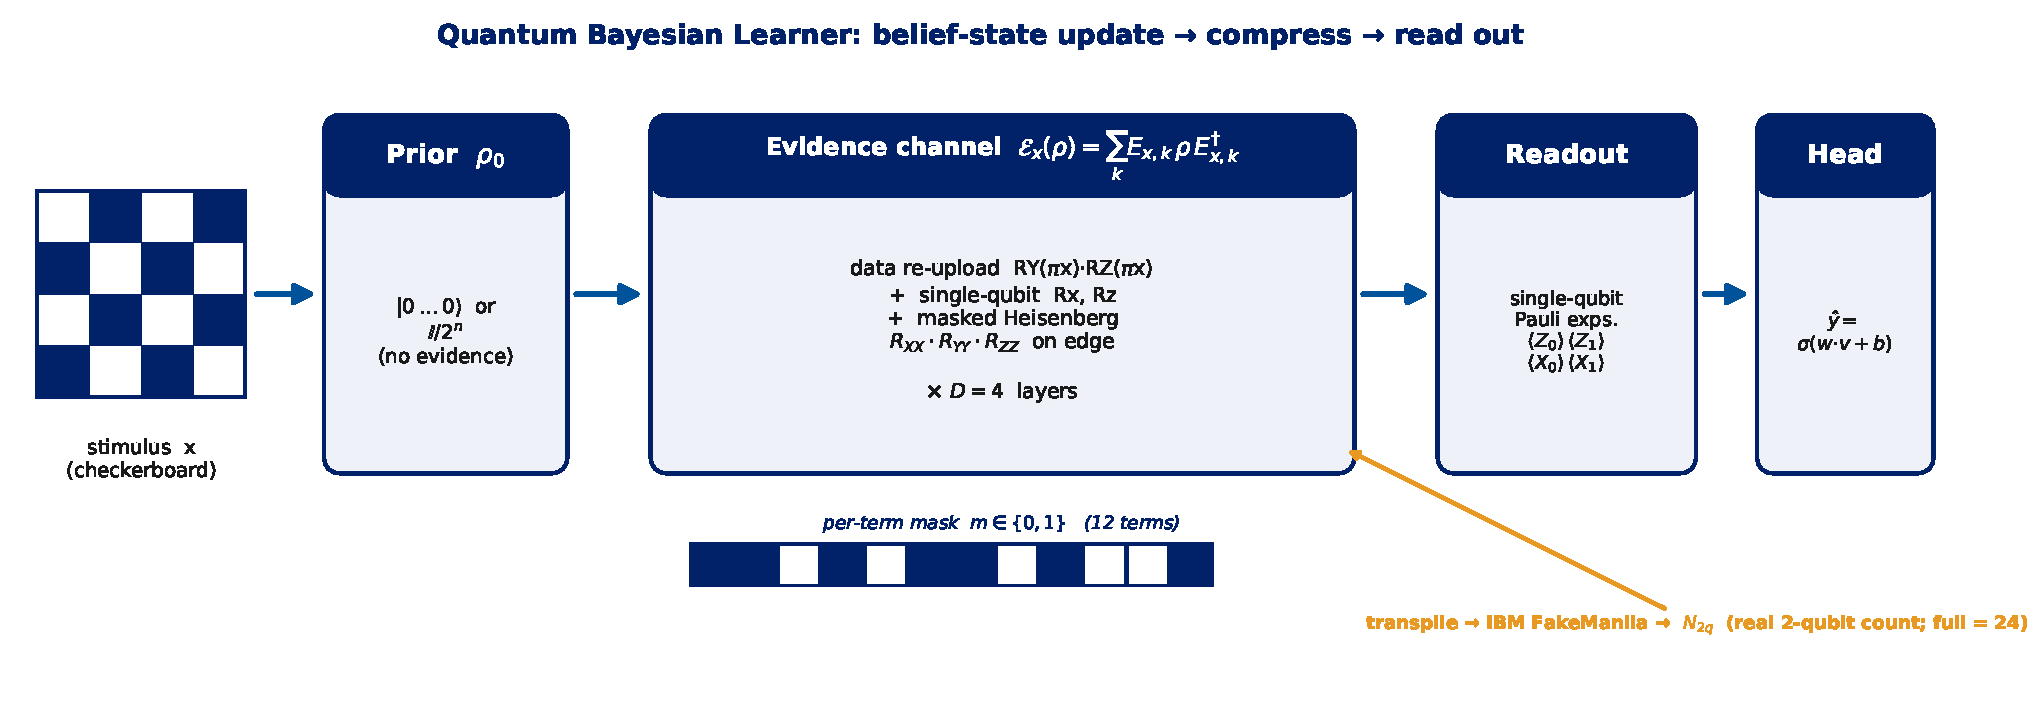
\includegraphics[width=\linewidth]{../assets/schematic.pdf}
\figcap{Left$\to$right pipeline: stimulus $x$ $\to$ prior $\rho_0$ $\to$ masked
Heisenberg evidence channel ($\times D{=}4$) $\to$ single-qubit Pauli readout $\to$
trainable head. The 12-cell mask gates the entanglers; transpiling to IBM FakeManila
yields the real two-qubit cost $N_{2q}$.}
\end{wbox}
\begin{cbox}
\begin{itemize}
  \item Belief = state $\rho$ on a \tl{2-qubit} register; prior $\rho_0$ = ``no
        evidence yet.'' A stimulus $x$ updates belief via a \tl{CPTP evidence channel}
        $\mathcal{E}_x(\rho)=\sum_k E_{xk}\,\rho\,E_{xk}^{\dagger}$.
  \item Update circuit = \tl{hardware-efficient ansatz}: data re-uploading
        + per-layer single-qubit $R_x,R_z$ + \tl{Heisenberg entanglers}
        $U_{ij}=\exp[-i(\alpha X_iX_j+\beta Y_iY_j+\gamma Z_iZ_j)]$ as native
        $R_{XX},R_{YY},R_{ZZ}$. Depth \tl{$D=4$}, 2 re-uploads.
  \item \tl{Readout: single-qubit Pauli expectations}
        $v=(\langle Z_0\rangle,\langle Z_1\rangle,\langle X_0\rangle,\langle X_1\rangle)$
        $\to$ trainable head $\hat{y}=\sigma(w\!\cdot\!v+b)$. Single-qubit-only readout
        means \tl{entanglement is the ONLY way to carry feature interaction} — the
        two-qubit budget literally bounds the learner's capacity.
  \item Two realizations, same conclusions: a fast \tl{pure-state} model and a literal
        \tl{mixed-state density matrix} (maximally mixed prior $I/2^n$, non-unital
        Lüders/POVM evidence filter + amplitude damping, Bayesian trace renormalization).
\end{itemize}
\end{cbox}

\secbar{3}{Method — mask, real cost, greedy compression}
\begin{cbox}
\begin{itemize}
  \item \tl{Per-term binary mask} $m_{\ell,p}\in\{0,1\}$ over $p\in\{XX,YY,ZZ\}$ in each
        of $D{=}4$ layers $\Rightarrow$ \tl{12 maskable terms} ($R_{PP}(0)=I$ when off).
  \item \tl{Hardware-aware cost $N_{2q}$} = real post-transpile two-qubit gate count on
        IBM \tl{FakeManila} (5-qubit, includes SWAPs), from Qiskit's transpiler. Full
        circuit $\Rightarrow$ \tl{$N_{2q}=24$} (each active Heisenberg term = 2 CNOTs).
  \item \tl{Objective:}\ \ $\displaystyle L(\theta,m)=\tfrac{1}{N}\sum_k
        \mathrm{BCE}(y_k,\hat{y})+\lambda\,N_{2q}(m).$
  \item \tl{Greedy structured pruning:} from the full circuit, repeatedly drop the term
        whose removal least increases training cross-entropy, \tl{warm-start retrain} —
        tracing the accuracy-vs-$N_{2q}$ \tl{frontier} from 24 down to 0.
  \item Exact \tl{JAX autodiff} (no parameter-shift / finite differences); statevector
        verified \tl{bit-for-bit vs Qiskit} ($|1-\mathrm{fidelity}|\approx4\times10^{-16}$).
\end{itemize}
\vspace{4pt}
\textbf{\color{dukenavy}Task — controllable difficulty knob.}
\begin{itemize}
  \item \tl{Checkerboard} categorization:
        $y=(\lfloor f x_0\rfloor+\lfloor f x_1\rfloor)\bmod 2$, stimuli in $[0,1]^2$.
  \item Difficulty $f$: \tl{$f{=}2$ easy / $f{=}3$ medium / $f{=}4$ hard}. 200 stimuli,
        70/30 split, balanced $\Rightarrow$ \tl{chance $=0.5$}. The rule depends on the
        \tl{joint} features — needing interaction only entanglement can supply.
\end{itemize}
\end{cbox}

\end{minipage}%
\hspace{\sepw}%
\begin{minipage}[t]{\colw}
%================================ COLUMN 2 ====================================

\secbar{4}{Result 1 — The capacity boundary}
\begin{wbox}
\centering
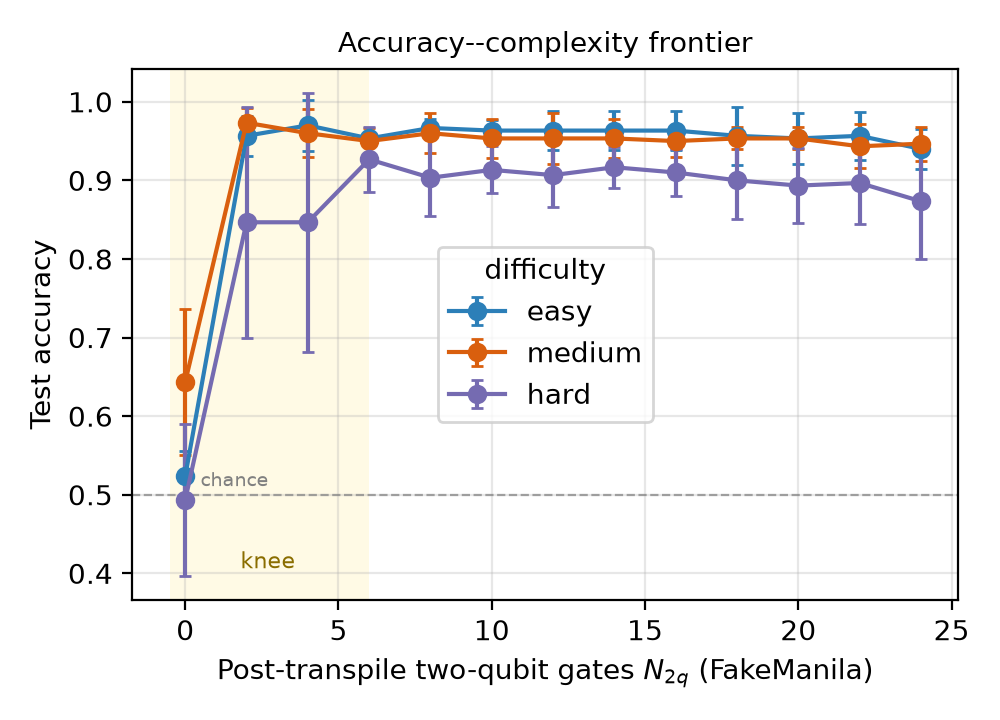
\includegraphics[width=\linewidth]{../figures/fig_frontier_family.png}
\figcap{Accuracy–complexity frontier across difficulties. Flat above the knee;
collapse toward chance at $N_{2q}=0$.}
\end{wbox}
\begin{cbox}
\begin{itemize}
  \item Above chance at all nonzero budgets (easy/medium $\approx$ \tl{0.95–0.97},
        hard $\approx$ \tl{0.87–0.93}); frontier \tl{nearly flat} — most entangling
        structure is \tl{redundant}.
  \item At \tl{$N_{2q}=0$} all difficulties \tl{collapse toward chance} (0.52 easy,
        0.64 medium, 0.49 hard) — some entanglement is \tl{necessary}, but far less
        than the full circuit.
  \item Hard task (not saturated): accuracy \tl{peaks at intermediate cost}
        (\tl{0.927 @ $N_{2q}{=}6$}) and is lower for the full circuit
        (\tl{0.873 @ $N_{2q}{=}24$}) — moderate compression acts as a capacity-control
        \tl{regularizer}.
\end{itemize}
\end{cbox}

\secbar{5}{Result 2 — Structure beats count}
\begin{wbox}
\centering
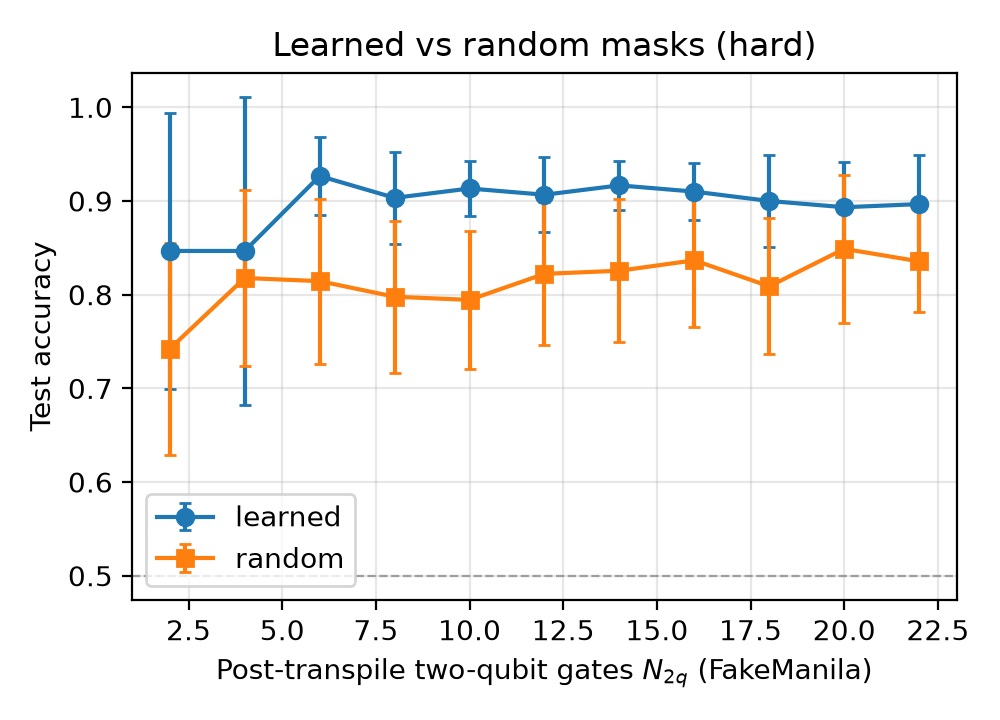
\includegraphics[width=\linewidth]{../figures/fig_mask_ablation.png}
\figcap{Learned (greedy) masks vs random masks at matched $N_{2q}$, hard task.}
\end{wbox}
\begin{cbox}
\begin{itemize}
  \item Learned masks vs \tl{random masks at matched $N_{2q}$}: learned wins at
        \tl{every} budget by \tl{$\sim$6–12 points}.
  \item Per seed: learned beats random in \tl{49 / 55} paired (seed,\,budget)
        comparisons, mean advantage \tl{$+0.083$}, one-sided Wilcoxon \tl{$p<10^{-7}$}.
  \item $\Rightarrow$ \tl{Which} entanglers you keep matters, not just how many.
\end{itemize}
\vspace{8pt}
{\centering
\renewcommand{\arraystretch}{1.28}
\setlength{\tabcolsep}{14pt}
\begin{tabular}{>{\centering\arraybackslash}p{2.6cm}
                >{\centering\arraybackslash}p{3.2cm}
                >{\centering\arraybackslash}p{3.2cm}
                >{\centering\arraybackslash}p{3.0cm}}
\arrayrulecolor{dukenavy}\toprule
\rowcolor{dukenavy}
\textbf{\color{white}$N_{2q}$} & \textbf{\color{white}Learned} &
\textbf{\color{white}Random} & \textbf{\color{white}$\Delta$}\\
\midrule
2  & 0.847 & 0.742 & \textbf{+0.104}\\
6  & \textbf{0.927} & 0.814 & \textbf{+0.112}\\
10 & 0.913 & 0.794 & \textbf{+0.119}\\
14 & 0.917 & 0.826 & \textbf{+0.091}\\
18 & 0.900 & 0.809 & \textbf{+0.091}\\
22 & 0.897 & 0.836 & \textbf{+0.061}\\
\bottomrule
\end{tabular}\par}
\vspace{6pt}
{\footnotesize\color{dukeroyal}\textit{Hard task — learned vs random, mean accuracy,
5 seeds.}}
\vspace{6pt}

\begin{tcolorbox}[enhanced, sharp corners, boxrule=0pt, frame hidden,
    colback=dukenavy!8, left=10pt,right=10pt,top=8pt,bottom=8pt, width=\linewidth]
  \color{dukenavy}\small\textbf{$\lambda$-sweep (hard):}
  $\lambda{=}0\!\to\!N_{2q}\,9.6$, acc 0.923;\ \
  $\lambda{=}0.04\!\to\!N_{2q}\,3.2$, acc 0.933;\ \
  $\lambda{=}0.15\!\to\!N_{2q}\,1.6$, acc 0.823.
  \textit{Sheds $\sim$2/3 of 2-qubit gates for free, $>$90\% at modest cost.}
\end{tcolorbox}
\end{cbox}

\secbar{6}{Robustness — not an artifact}
\begin{cbox}
\begin{itemize}
  \item \tl{Device noise model} (FakeManila, 4096 shots, 5 seeds): noisy accuracy tracks
        the noiseless frontier within a few \% at every budget — savings genuine net of
        noise.
  \item \tl{Density-matrix model} (genuine mixed state, non-unital channel): reproduces
        every finding — flat frontier, collapse at $N_{2q}=0$, hard peak
        \tl{0.88 @ 6 vs 0.87 @ 24}, learned $>$ random (mean \tl{$+0.043$}).
  \item \tl{Classical baselines} (identical splits, 5 seeds): logistic regression at
        chance on every level; RBF-SVM \& MLP fall monotonically easy$\to$hard. Best
        compressed QBL: \tl{easy 0.970, medium 0.973, hard 0.927}.
\end{itemize}
\end{cbox}

\end{minipage}%
\hspace{\sepw}%
\begin{minipage}[t]{\colw}
%================================ COLUMN 3 ====================================

\secbar{7}{Result 3 — On REAL hardware, compression becomes NECESSARY}
\begin{amberbox}
\centering
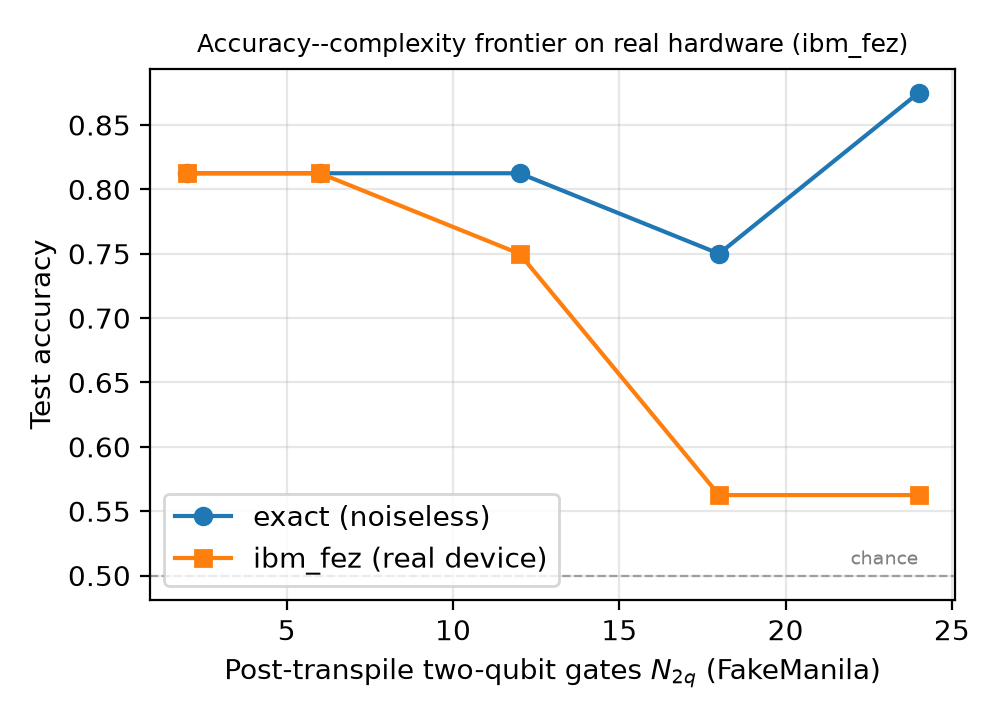
\includegraphics[width=\linewidth]{../figures/fig_hardware_frontier.png}
\figcap{Centerpiece. Trained circuits on physical IBM \texttt{ibm\_fez} (156-qubit
Heron). In simulation the frontier is flat; on hardware it falls monotonically.}
\vspace{4pt}
\begin{flushleft}\color{inkblack}
\begin{itemize}
  \item Hard task, 5 device budgets, \tl{16 test stimuli @ 2048 shots} (endpoints:
        40 stimuli @ 4096 shots).
  \item On hardware accuracy \tl{falls monotonically} with $N_{2q}$:
        \tl{0.81 @ $N_{2q}{=}2,6$ $\to$ 0.75 @ 12 $\to$ collapses to 0.56}
        (near chance) \tl{@ 18,24}.
  \item Endpoint confirmation: \tl{full circuit 0.60} (sim 0.95) vs
        \tl{compressed 0.83} (sim 0.93).
\end{itemize}
\end{flushleft}
\vspace{2pt}
\begin{tcolorbox}[enhanced, sharp corners, boxrule=0pt, frame hidden,
    colback=dukeamber!15, left=12pt,right=12pt,top=10pt,bottom=10pt, width=\linewidth]
  \color{dukenavy}\bfseries\large
  Takeaway: On real NISQ hardware, hardware-aware compression of the quantum Bayesian
  learner is not merely economical but \textcolor{dukeamber}{NECESSARY} — surplus
  entangling capacity is actively harmful, and task-aware pruning is what makes the
  learner usable at all.
\end{tcolorbox}
\end{amberbox}

\secbar{8}{Key takeaways}
\begin{cbox}
\begin{itemize}
  \item Most entanglement is \tl{redundant} — sheds $\sim$\tl{2/3} of two-qubit gates
        for \tl{free}, \tl{$>$90\%} at modest cost.
  \item Entanglement is \tl{necessary} — removing all of it collapses the learner to
        chance: a concrete \tl{capacity boundary}.
  \item \tl{Structure beats count} — learned masks beat random at every matched budget.
  \item \tl{On real hardware, compression is what makes the learner work at all.}
\end{itemize}
\vspace{4pt}
{\small\textbf{\color{dukenavy}Future work.} Multi-qubit belief registers \& higher-dim
stimuli; richer non-unital evidence channels; hardware-aware objectives weighting depth,
coherence \& native fidelity; feeding measured device error rates back into the
compression objective.}
\end{cbox}

\secbar{}{References \& links}
\begin{cbox}
{\footnotesize\sloppy
\textbf{\color{dukenavy}Key references}\\[3pt]
[1] Busemeyer \& Bruza, \textit{Quantum Models of Cognition and Decision}, 2012.\\[2pt]
[2] Pothos \& Chater, ``A simplicity principle in unsupervised human categorization,''
    \textit{Cogn. Psych.}, 2002.\\[2pt]
[3] Kandala et al., ``Hardware-efficient VQE\dots,'' \textit{Nature}, 2017.\\[2pt]
[4] Preskill, ``Quantum computing in the NISQ era and beyond,'' \textit{Quantum}, 2018.\\[2pt]
[5] Cerezo et al., ``Variational quantum algorithms,'' \textit{Nat. Rev. Phys.}, 2021.\\[2pt]
[6] Sim et al., ``Adaptive pruning-based optimization of PQCs,''
    \textit{Quantum Sci. Technol.}, 2021.
\par}
\vspace{10pt}
\hrule height 0.8pt
\vspace{10pt}
\begin{minipage}[c]{0.30\linewidth}
  
\includegraphics[width=\linewidth]{../assets/repo_qr.png}
\end{minipage}\hfill
\begin{minipage}[c]{0.66\linewidth}
  {\small
  \textbf{\color{dukenavy}Repository}\\
  github.com/zoraizmohammad/qb-learner-compression\\[8pt]
  \textbf{\color{dukenavy}Acknowledgments}\\
  Device runs used IBM Quantum services. The author thanks Duke University's Pratt
  School of Engineering.\\[8pt]
  \textbf{\color{dukenavy}Contact}\\
  Mohammad Zoraiz $\cdot$ mz248@duke.edu}
\end{minipage}
\end{cbox}

\end{minipage}%
\end{textblock*}

\end{frame}
\end{document}
